\documentclass{beamer}
\newcommand{\plt}{../../plots}
\usepackage{multimedia}
\usepackage{hyperref}
\usepackage{amsmath}
\usepackage{amssymb, amsthm}
\usepackage{bm}
% \addmediapath{\plt}

\mode<presentation> {

% The Beamer class comes with a number of default slide themes
% which change the colors and layouts of slides. Below this is a list
% of all the themes, uncomment each in turn to see what they look like.

%\usetheme{default}
%\usetheme{AnnArbor}
%\usetheme{Antibes}
%\usetheme{Bergen}
%\usetheme{Berkeley}
%\usetheme{Berlin}
%\usetheme{Boadilla}
\usetheme{CambridgeUS}
%\usetheme{Copenhagen}
%\usetheme{Darmstadt}
%\usetheme{Dresden}
%\usetheme{Frankfurt}
%\usetheme{Goettingen}
%\usetheme{Hannover}
%\usetheme{Ilmenau}
%\usetheme{JuanLesPins}
%\usetheme{Luebeck}
% \usetheme{Madrid}
%\usetheme{Malmoe}
%\usetheme{Marburg}
%\usetheme{Montpellier}
%\usetheme{PaloAlto}
%\usetheme{Pittsburgh}
%\usetheme{Rochester}
%\usetheme{Singapore}
%\usetheme{Szeged}
%\usetheme{Warsaw}

% As well as themes, the Beamer class has a number of color themes
% for any slide theme. Uncomment each of these in turn to see how it
% changes the colors of your current slide theme.

%\usecolortheme{albatross}
%\usecolortheme{beaver}
%\usecolortheme{beetle}
%\usecolortheme{crane}
%\usecolortheme{dolphin}
%\usecolortheme{dove}
%\usecolortheme{fly}
%\usecolortheme{lily}
%\usecolortheme{orchid}
%\usecolortheme{rose}
%\usecolortheme{seagull}
%\usecolortheme{seahorse}
%\usecolortheme{whale}
%\usecolortheme{wolverine}

%\setbeamertemplate{footline} % To remove the footer line in all slides uncomment this line
%\setbeamertemplate{footline}[page number] % To replace the footer line in all slides with a simple slide count uncomment this line

%\setbeamertemplate{navigation symbols}{} % To remove the navigation symbols from the bottom of all slides uncomment this line
}

\usepackage{graphicx} % Allows including images
\usepackage{booktabs} % Allows the use of \toprule, \midrule and \bottomrule in tables

%----------------------------------------------------------------------------------------
%   TITLE PAGE
%----------------------------------------------------------------------------------------
\setbeamertemplate{itemize items}[circle]
\setbeamertemplate{enumerate items}[circle]

\title[Motivic analysis]{Motivic analysis of neuronal signals} % The short title appears at the bottom of every slide, the full title is only on the title page

\author{Athul Vijayan} % Your name
\institute[DON Lab] % Your institution as it will appear on the bottom of every slide, may be shorthand to save space
{
IIT Madras \\ % Your institution for the title page
\medskip
\textit{athulvijayan6@gmail.com} % Your email address
}
\date{\today} % Date, can be changed to a custom date

\begin{document}

\begin{frame}
\titlepage % Print the title page as the first slide
\end{frame}


\begin{frame}
\frametitle{Overview}
\begin{itemize}
    \item How does neurons in Primary Visual Cortex (V1) behave?
    \item Motifs here refer to recurring patterns in the time-series response of neurons. Are there motifs in neuronal responses?
    \item What is similar in responses of two different neurons in a same mice?
    \item What is similar in responses of two neurons in different mices?
    \item What does these similarities mean?
\end{itemize}
\end{frame}

\begin{frame}
\frametitle{Experiment}
Virus expressing GCaMP6f was injected into the V1 of mice. mice were imaged under a 2-photon microscope while sinusoidal drifting gratings/video were presented on a computer screen placed 3 inches from the mouse (1 degree of visual space $\sim$ 21.3 pixels on the screen).
\begin{figure}
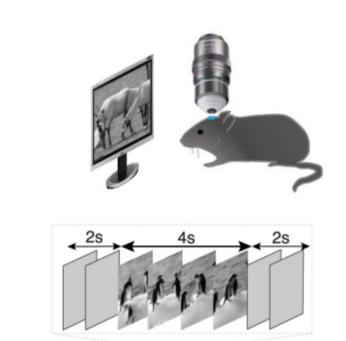
\includegraphics[width=0.4\linewidth]{img/exp.png}
\end{figure}
\end{frame}

\begin{frame}
\frametitle{Data}

\begin{columns}[c]
\column{.4\textwidth} % Left column and width
\begin{center}
    \href{run:img/sin.mp4}{
    
\includegraphics[width=0.5\linewidth]
    {img/grating_c.png}}
\end{center}
\column{.6\textwidth} % Right column and width
\begin{center}
    \href{run:img/ani.mp4}{
    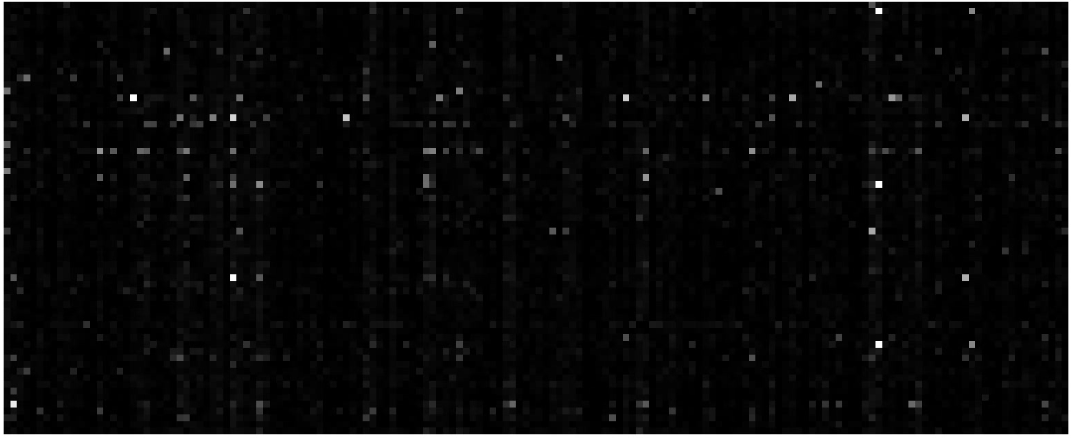
\includegraphics[width=0.5\linewidth]
    {img/resp_c.png}}
\end{center}
\end{columns}
\begin{figure}
\includegraphics[width=0.5\linewidth]{\plt/visualMain_meanPlot_2016_02_05_13_03_29.pdf}
\end{figure}
\end{frame}

\begin{frame}
\frametitle{Background}
\textbf{Orientation and Directional selectivity of neurons in V1}
\begin{itemize}
    \item Cells which respond to orientation of a contrasting visual stimuli. - simple cells
    \item Among the orientation selective cells, some cells are also sensitive to motion of the stimuli in a particular direction. - complex cells
    \item Orientation insensitive cells.
\end{itemize}
\textbf{Quantifying selectivity}
\begin{block}{Orientation selectivity index}
$$L_{ori} = \frac{\sum_{k} R(\theta_k) exp(2\theta_k)}{\sum_{k} R(\theta_k)}$$
\end{block}
\begin{block}{Directional selectivity index}
$$L_{dir} = \frac{\sum_{k} R(\theta_k) exp(\theta_k)}{\sum_{k} R(\theta_k)}$$
\end{block}
\end{frame}

\begin{frame}
\frametitle{Background}
\begin{columns}[c]
\column{.45\textwidth} % Left column and width
\begin{figure}
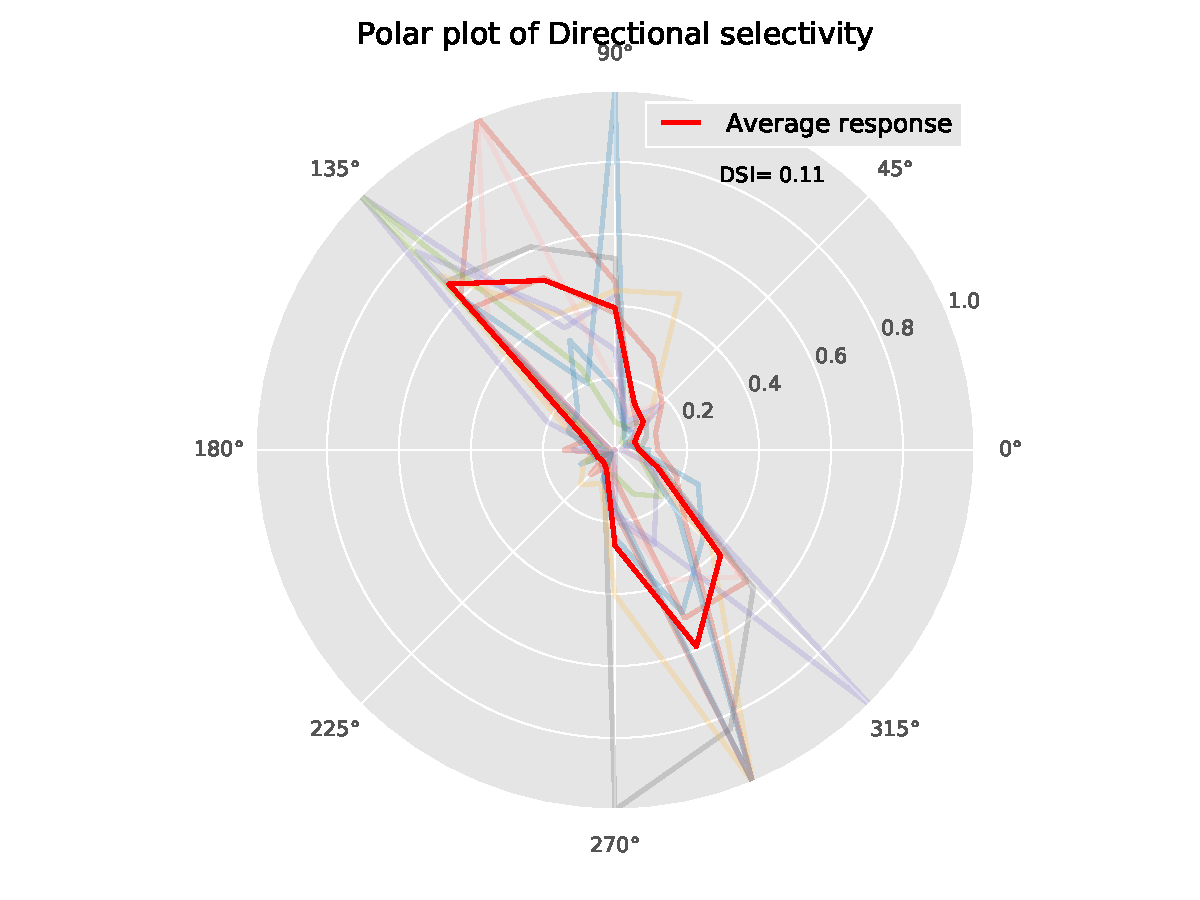
\includegraphics[width=\linewidth]{\plt/gratings_dirpolar_2016_04_24_14_08_33.pdf}
\end{figure}
\column{.5\textwidth} % Right column and width
\begin{figure}
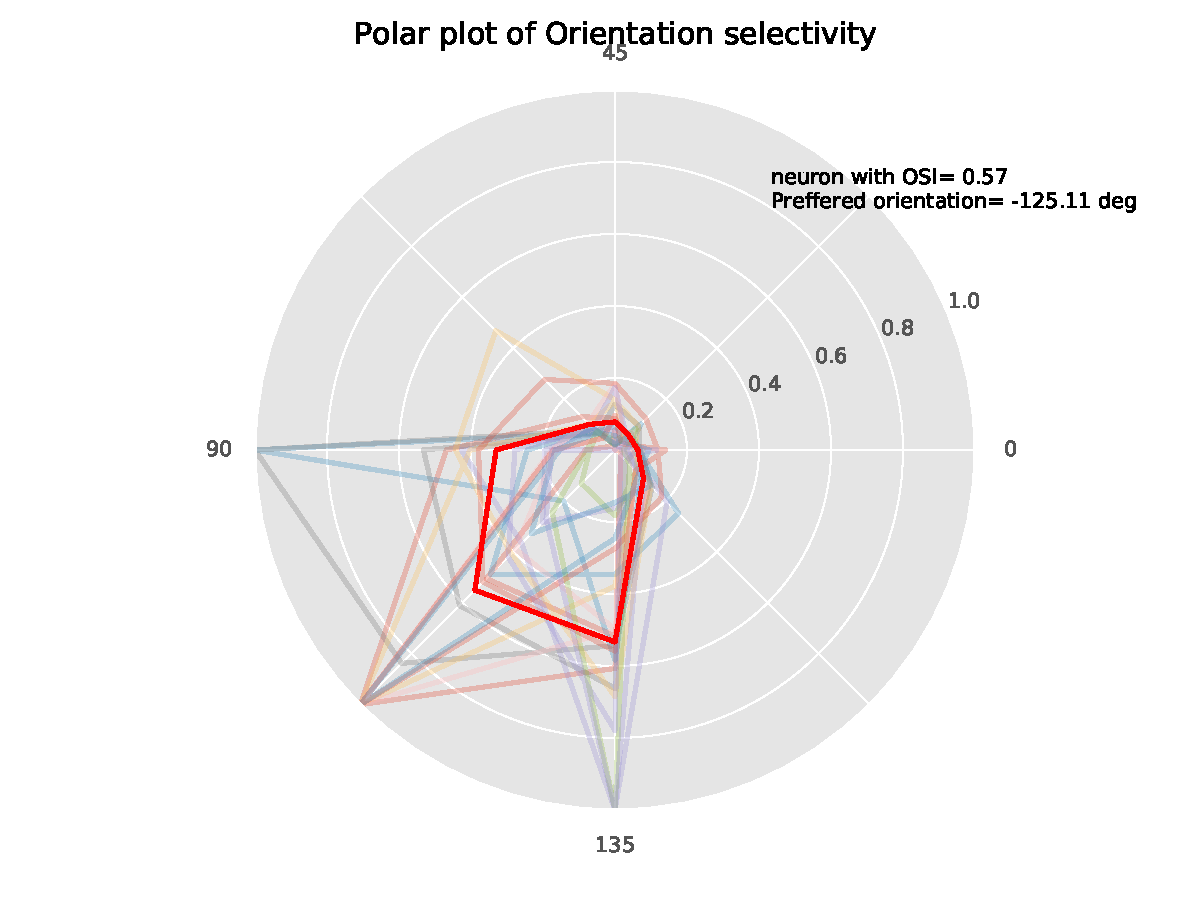
\includegraphics[width=\linewidth]{\plt/gratings_oripolar_2016_04_24_14_08_33.pdf}
\end{figure}
\end{columns}
\end{frame}

\begin{frame}
\frametitle{Reliability and correlation}
Response reliability to movie A ($R_A$ ) is
\begin{block}{Reliability Measure}
$$R_A = \frac{2}{T^2 - T}\sum_{i=1}^T \sum_{j=i+1}^T \rho(f_{i, A}, f_{j, A})$$
\end{block}
where $f_{i, A}$ is the response of neuron to $i^{th}$ trial of movie A and $\rho$ is the Pearson correlation.
\begin{columns}[c]
\column{.5\textwidth} % Left column and width
\textbf{Reliability measure is very low ($\sim 0.15$) for most of the neurons.}
\column{.45\textwidth} % Right column and width
\begin{figure}
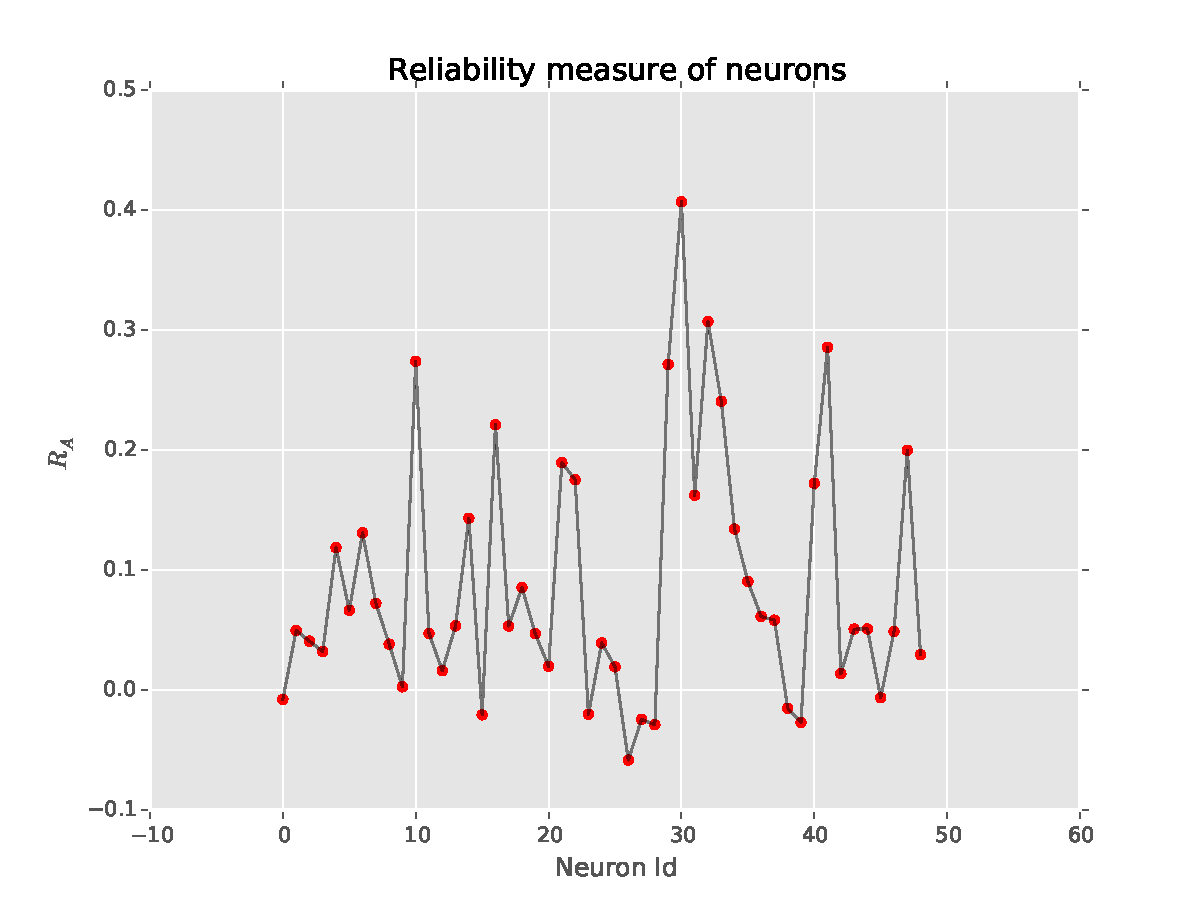
\includegraphics[width=.85\linewidth]{\plt/reliabMain_raPlot_2016_02_05_13_25_56.pdf}
\end{figure}
\end{columns}
\end{frame}

\begin{frame}
\frametitle{ACF analysis}
Having realized full time-series is not well correlated, We look for similar subsequences.
We do this by taking a frame from template signal and finding ACVF with target signal at various lags.
\begin{itemize}
    \item Heatmap of the ACF - a time vs lag vs ACF is created for analysis.
    \item For small window length ($\approx$ 15), the template is small. Such a small template does not satisfy as a motif. Also as the samples are less, estimate of sample correlation will be poor.
    \item For window lengths $\approx 30$ we see patterns. These shows that there are repeating subsequences in the response.
    \item \textbf{Common subsequences across different neurons are found.}
\end{itemize}
\end{frame}

\begin{frame}
\frametitle{ACFGram}
Same neuron, different trials.
\begin{columns}[c]

\column{.45\textwidth} % Left column and width
\begin{figure}
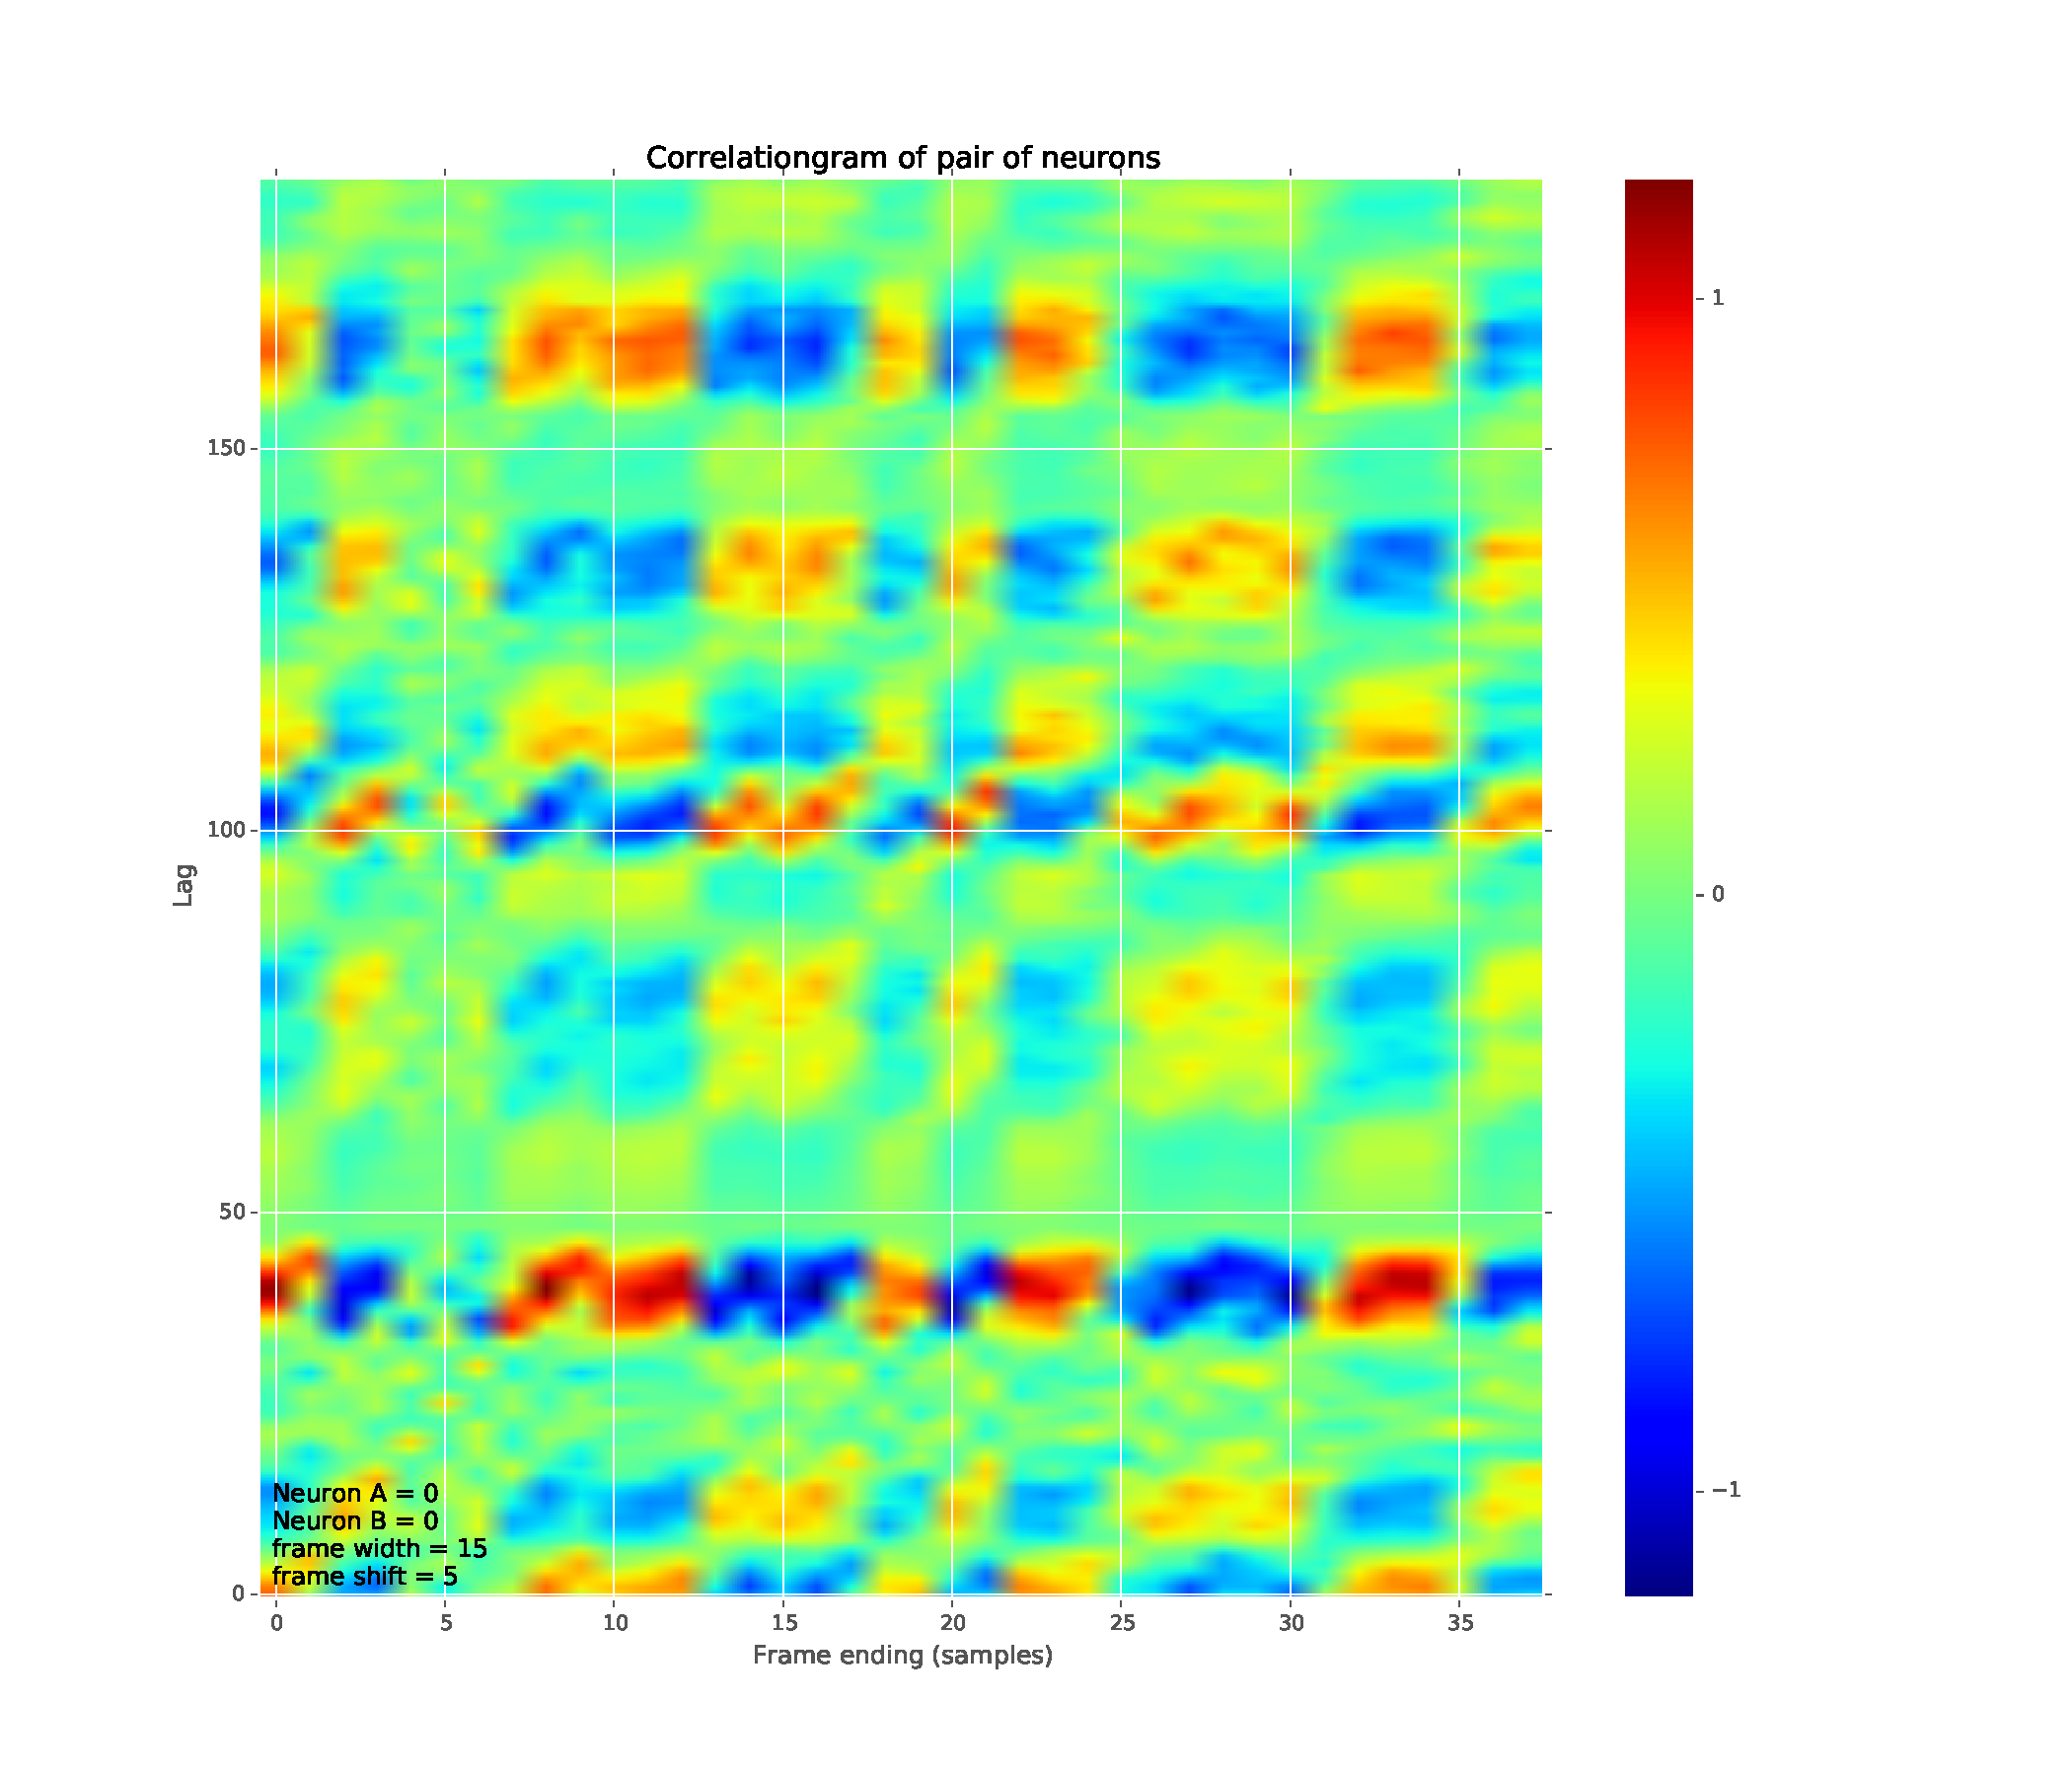
\includegraphics[width=\linewidth]{\plt/acfMain_corrGram_2016_02_05_16_49_00.pdf}
\end{figure}

\column{.5\textwidth} % Right column and width
\begin{figure}
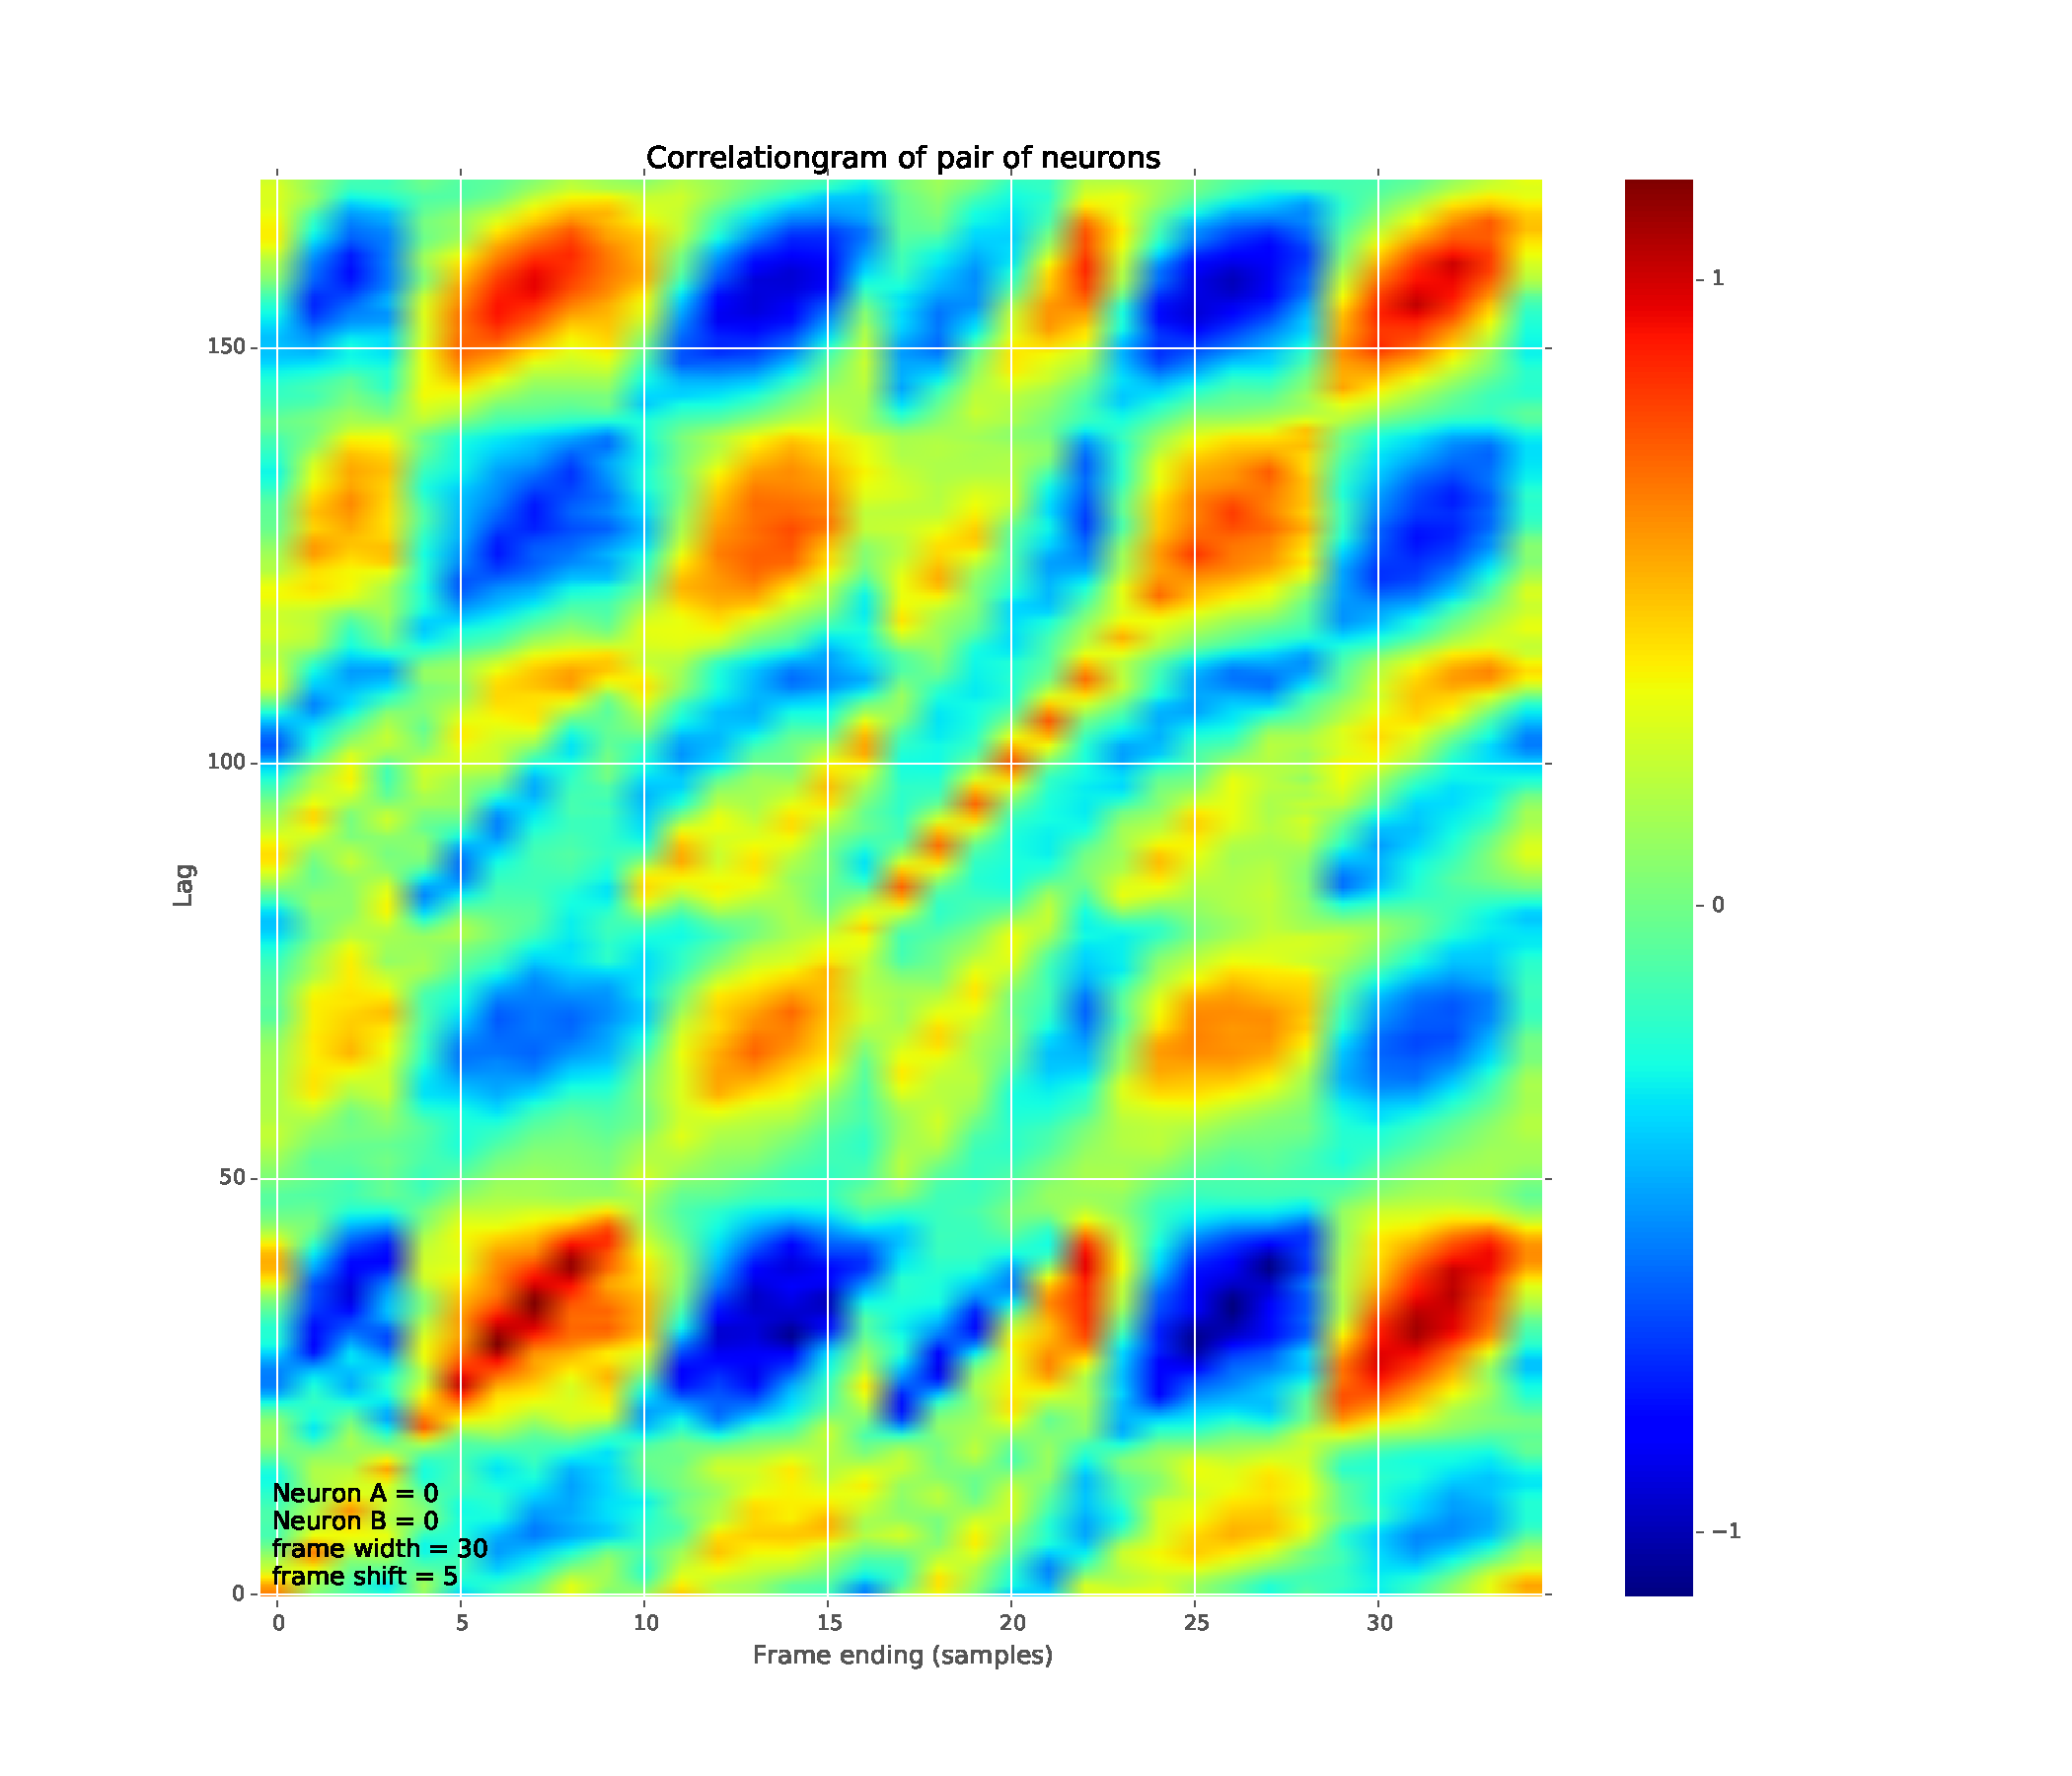
\includegraphics[width=\linewidth]{\plt/acfMain_corrGram_2016_02_05_16_49_10.pdf}
\end{figure}
\end{columns}
\end{frame}


\begin{frame}
\frametitle{ACFGram}
Different Neurons.
\begin{columns}[c]

\column{.45\textwidth} % Left column and width
\begin{figure}
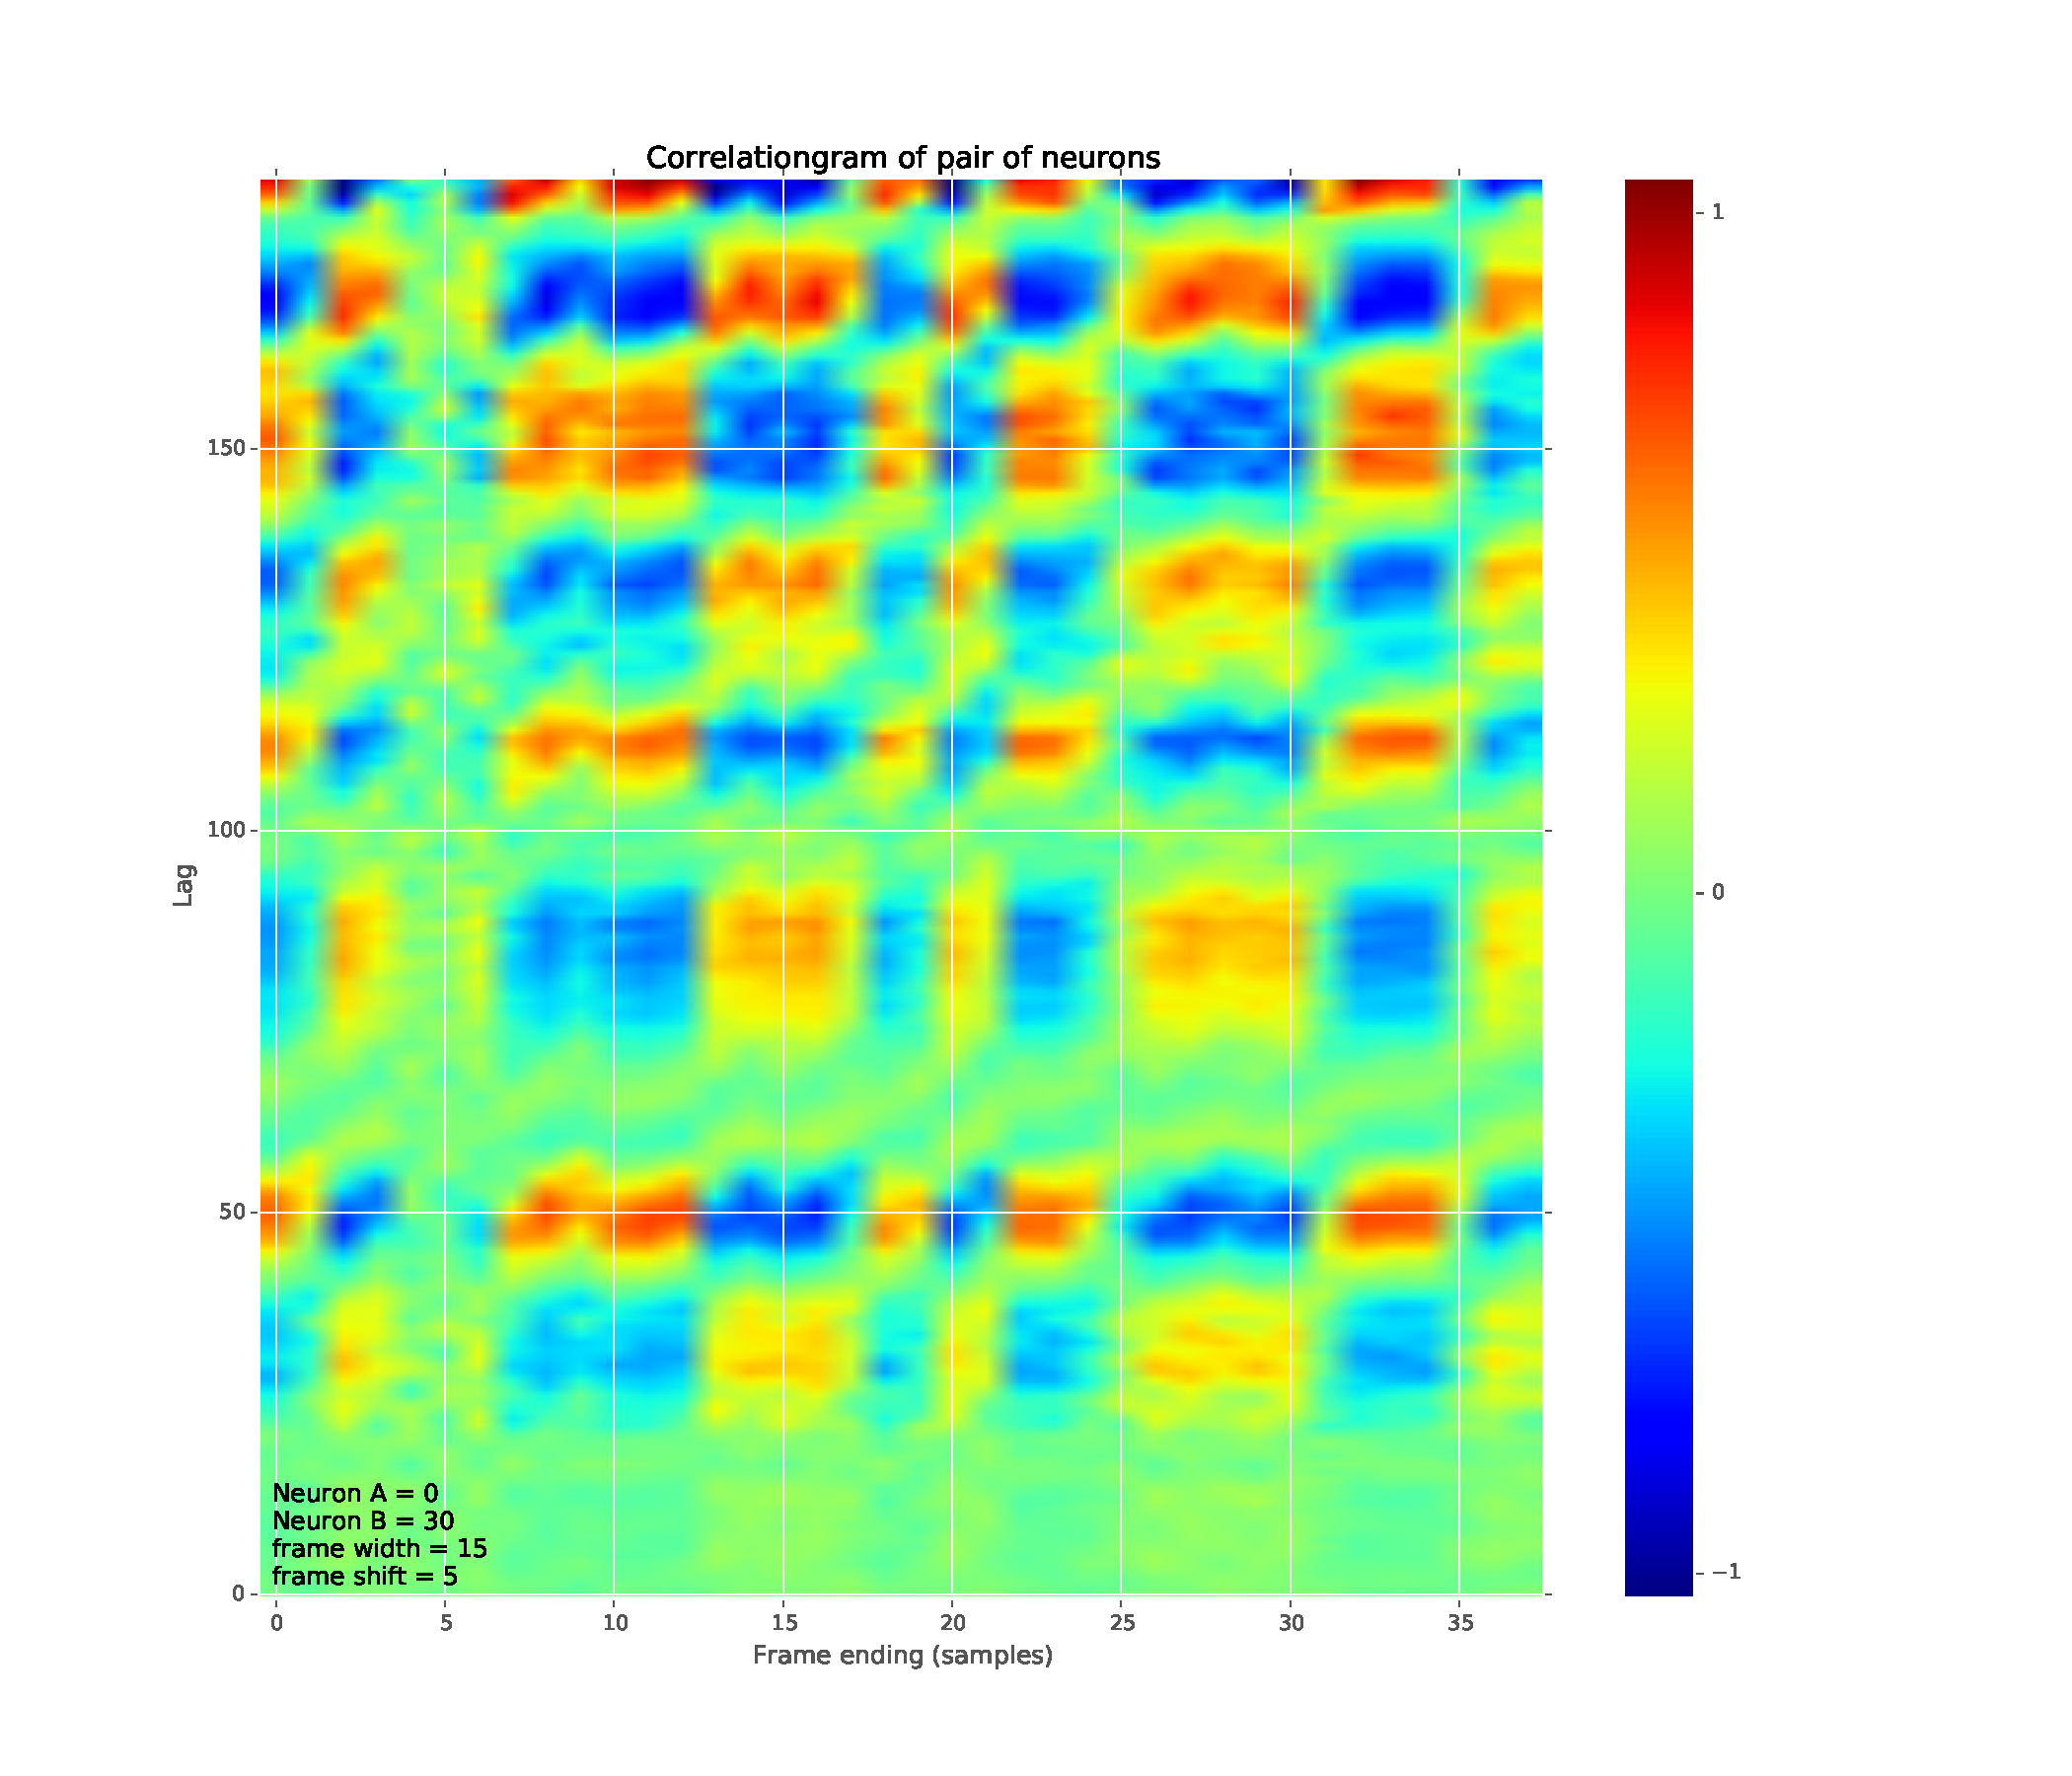
\includegraphics[width=\linewidth]{\plt/acfMain_corrGram_2016_02_05_16_45_22.pdf}
\end{figure}

\column{.5\textwidth} % Right column and width
\begin{figure}
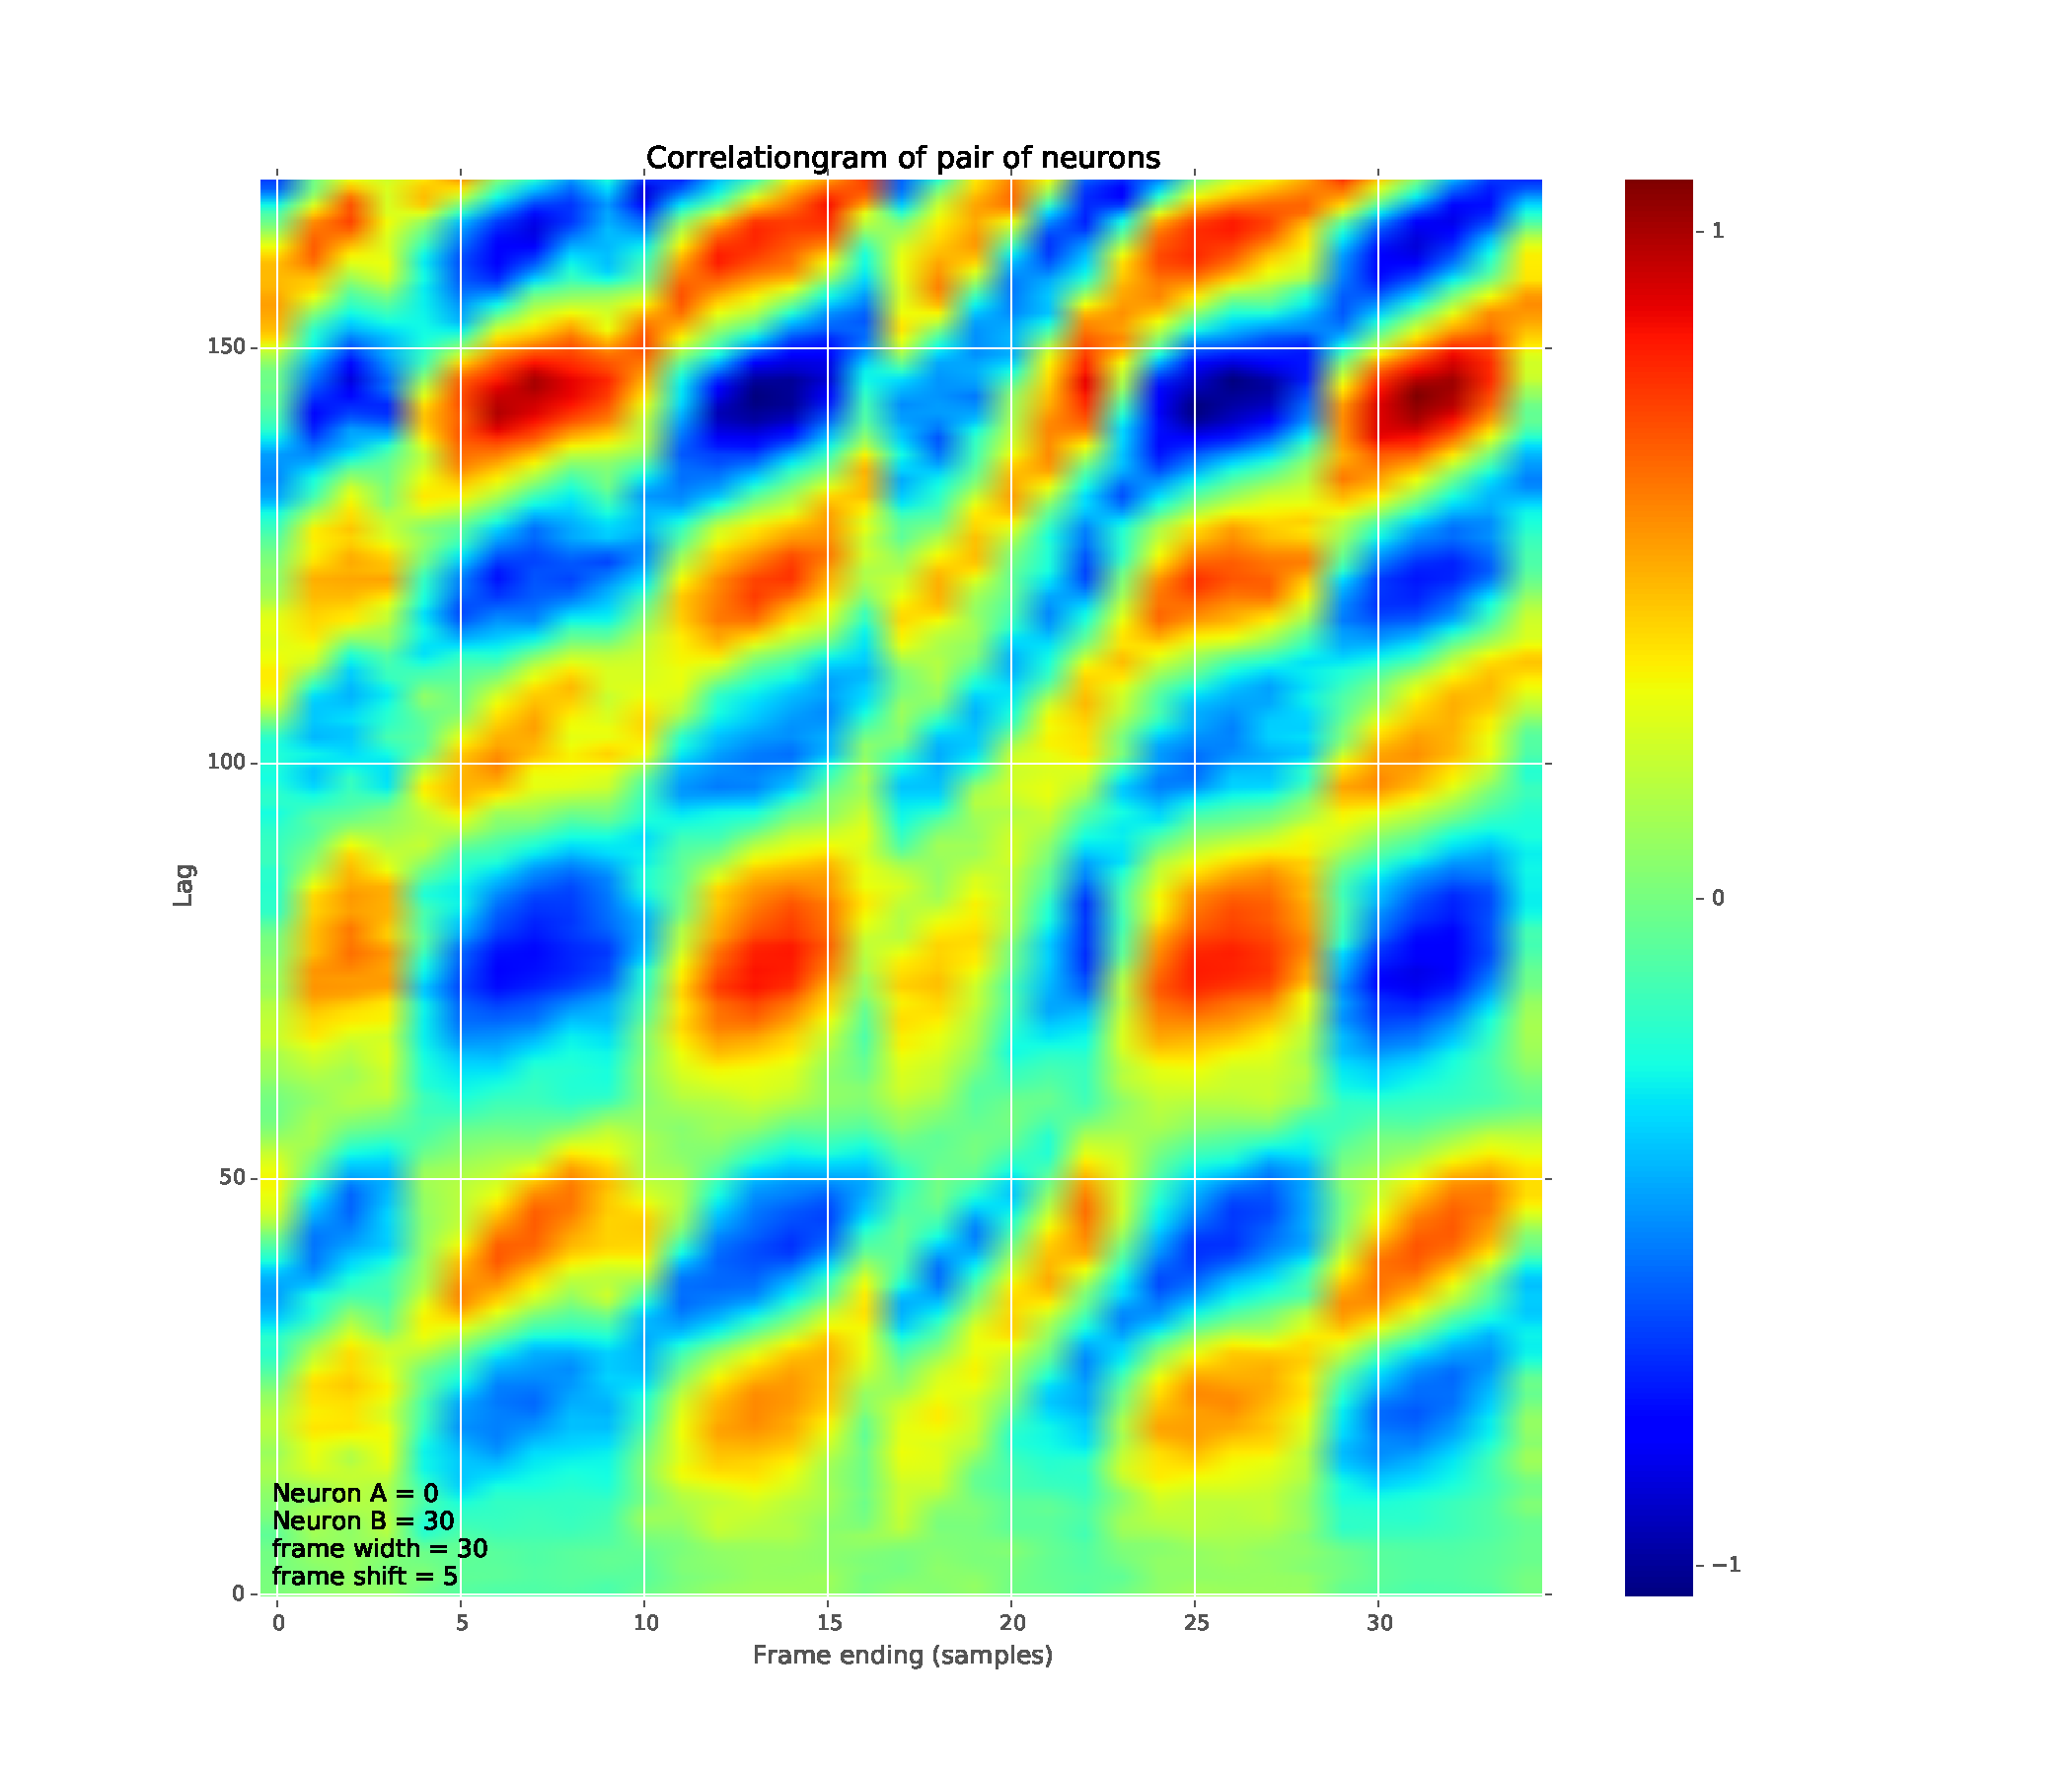
\includegraphics[width=\linewidth]{\plt/acfMain_corrGram_2016_02_05_16_45_38.pdf}
\end{figure}
\end{columns}
\end{frame}

\begin{frame}

\frametitle{Subsequence detection using RLCS}
\begin{block}{RLCS}
Let $\bm{X} = < x_1, x_2,\hdots, x_n ; x_i \in R >$ be template signal and $\bm{Y} = <y_1, y_2, \hdots, y_m ; y_m \in R>$ be the target signal.\\
Distance between sample $x_i$ and $y_j$ is 
$$dist(x_i, y_j) =  (x_i - y_j)^2$$
and RLCS problem is
$$
R\left(X_{i},Y_{j}\right) =
\begin{cases}
  \emptyset
& \mbox{ if }\ i = 0 \mbox{ or }  j = 0 \\
  \textrm{  } LCS\left(X_{i-1},Y_{j-1}\right) \frown x_{i}
& \mbox{ if } dist(x_i , y_j) < \tau_{dist} \\
  \mbox{max}\left(LCS\left(X_{i},Y_{j-1}\right),LCS\left(X_{i-1},Y_{j}\right)\right)
& \mbox{ if } dist(x_i , y_j) > \tau_{dist} \\
\end{cases}
$$
\end{block}
\end{frame}
\begin{frame}
    \frametitle{RLCS}
    \begin{block}{Score updates}
    \begin{itemize}
        \item For a sample match
        $$cost(i, j) = cost(i-1, j-1) + (1 - \frac{dist(x_i, y_j)}{\tau_{dist}})$$
        \item For a sample mismatch/ gap
        $$cost(i, j) = cost(i-1, j-1) - \delta$$
    \end{itemize}        
    \end{block}
    \begin{figure}
    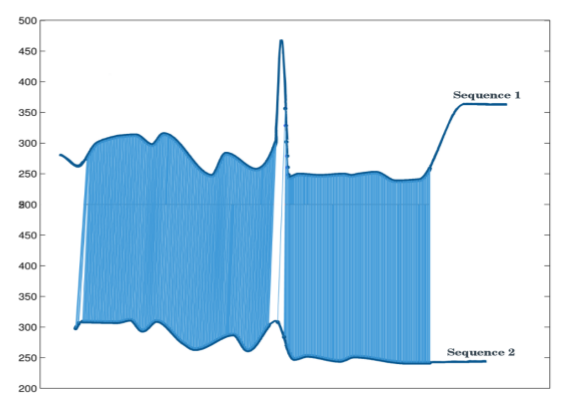
\includegraphics[width=0.35\linewidth]{img/rlcs.png}
    \end{figure}
\end{frame}

\begin{frame}
    \frametitle{Results}
    \textbf{Score matrix for same mice, different neurons}
    \begin{columns}[c]
    \column{.5\textwidth} % Left column and width
    \begin{figure}
    \includegraphics[width=\linewidth]{\plt/lcssMain_backtrack_2016_03_08_07_07_54.pdf}
    \end{figure}

    \column{.5\textwidth} % Right column and width
    \begin{figure}
    \includegraphics[width=\linewidth]{\plt/rlcsMain_backtrack_2016_04_06_12_54_14.pdf}
    \end{figure}
    \end{columns}
\end{frame}
\begin{frame}
    \frametitle{Results}
    \textbf{Longest common subsequence extracted from two neurons in same mice.}
    \begin{columns}[c]
    \column{.5\textwidth} % Left column and width
    \begin{figure}
    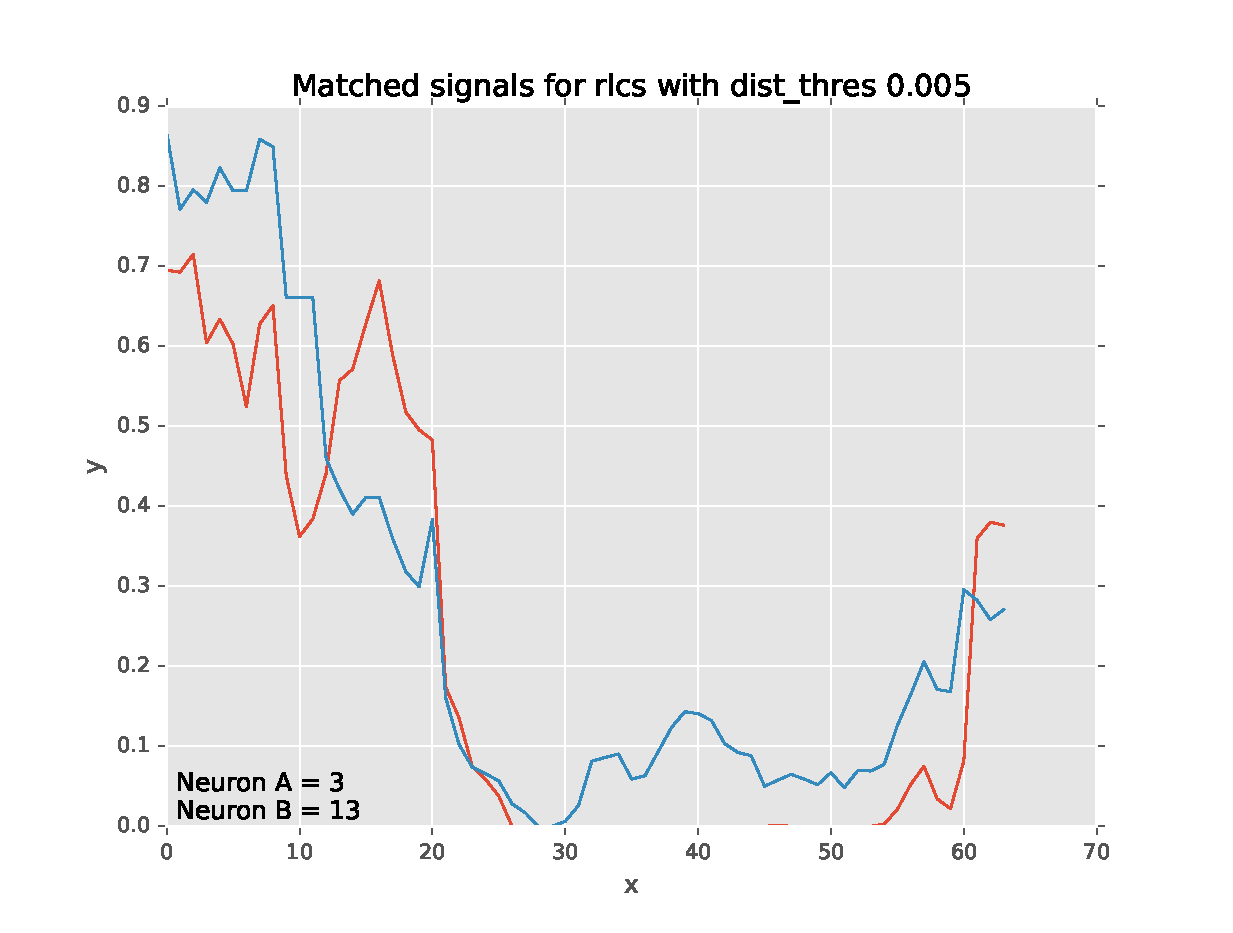
\includegraphics[width=\linewidth]{img/rlcsMain_getSegs_2016_04_06_10_23_00}
    \end{figure}

    \column{.5\textwidth} % Right column and width
    \begin{figure}
    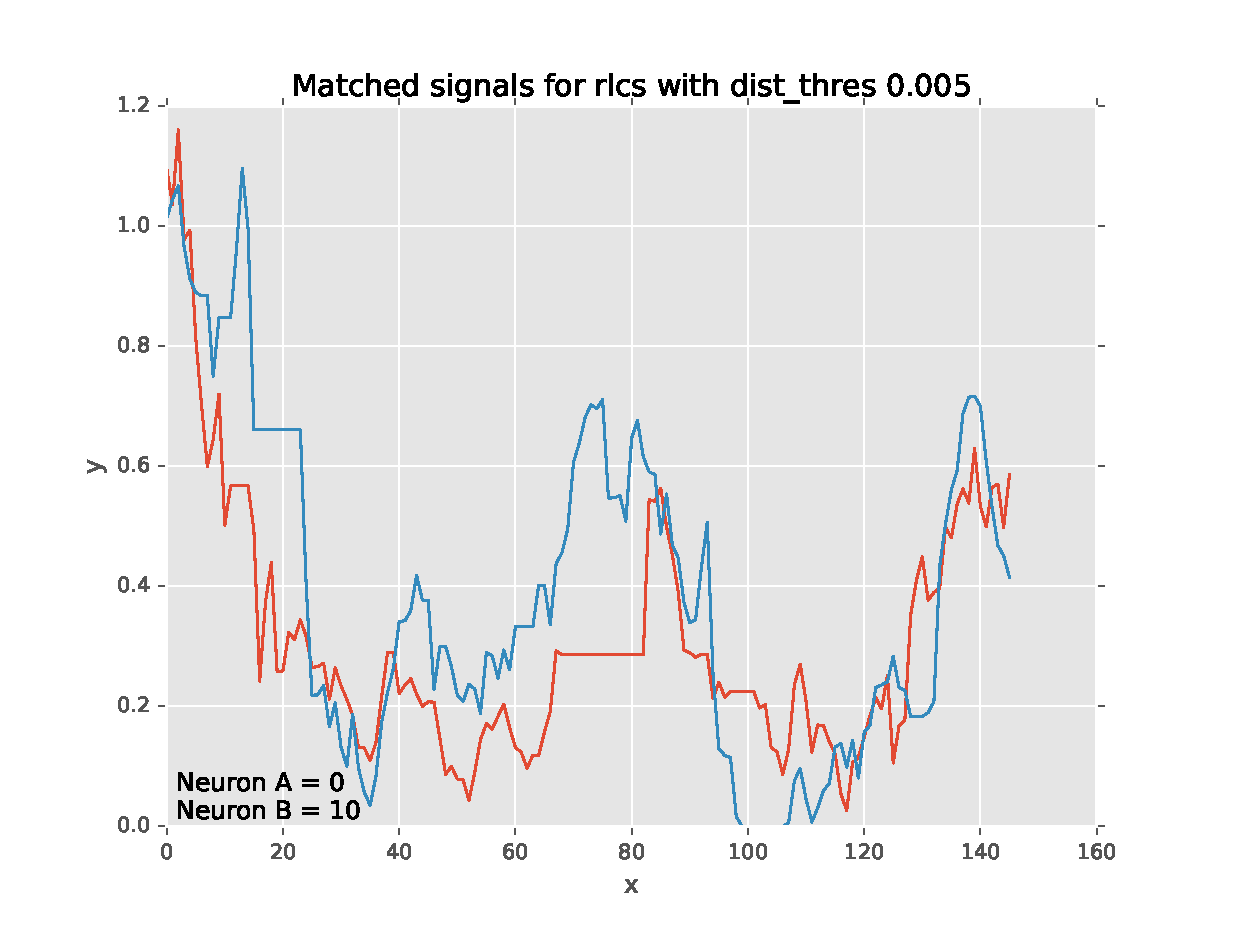
\includegraphics[width=\linewidth]{img/rlcsMain_getSegs_2016_04_06_10_22_55}
    \end{figure}
    \end{columns}
\end{frame}

\begin{frame}
    \frametitle{Results}
    \textbf{Score matrix for Different mice}
    \begin{columns}[c]
    \column{.5\textwidth} % Left column and width
    \begin{figure}
    \includegraphics[width=\linewidth]{\plt/rlcsMain_backtrack_2016_04_12_08_09_51.pdf}
    \end{figure}
    \column{.5\textwidth} % Right column and width
    \begin{figure}
    \includegraphics[width=\linewidth]{\plt/rlcsMain_backtrack_2016_04_12_08_12_31.pdf}
    \end{figure}
    \end{columns}
\end{frame}
\begin{frame}
    \frametitle{Results}
    \textbf{Longest common subsequence extracted from two neurons in different mice.}
    \begin{columns}[c]
    \column{.5\textwidth} % Left column and width
    \begin{figure}
    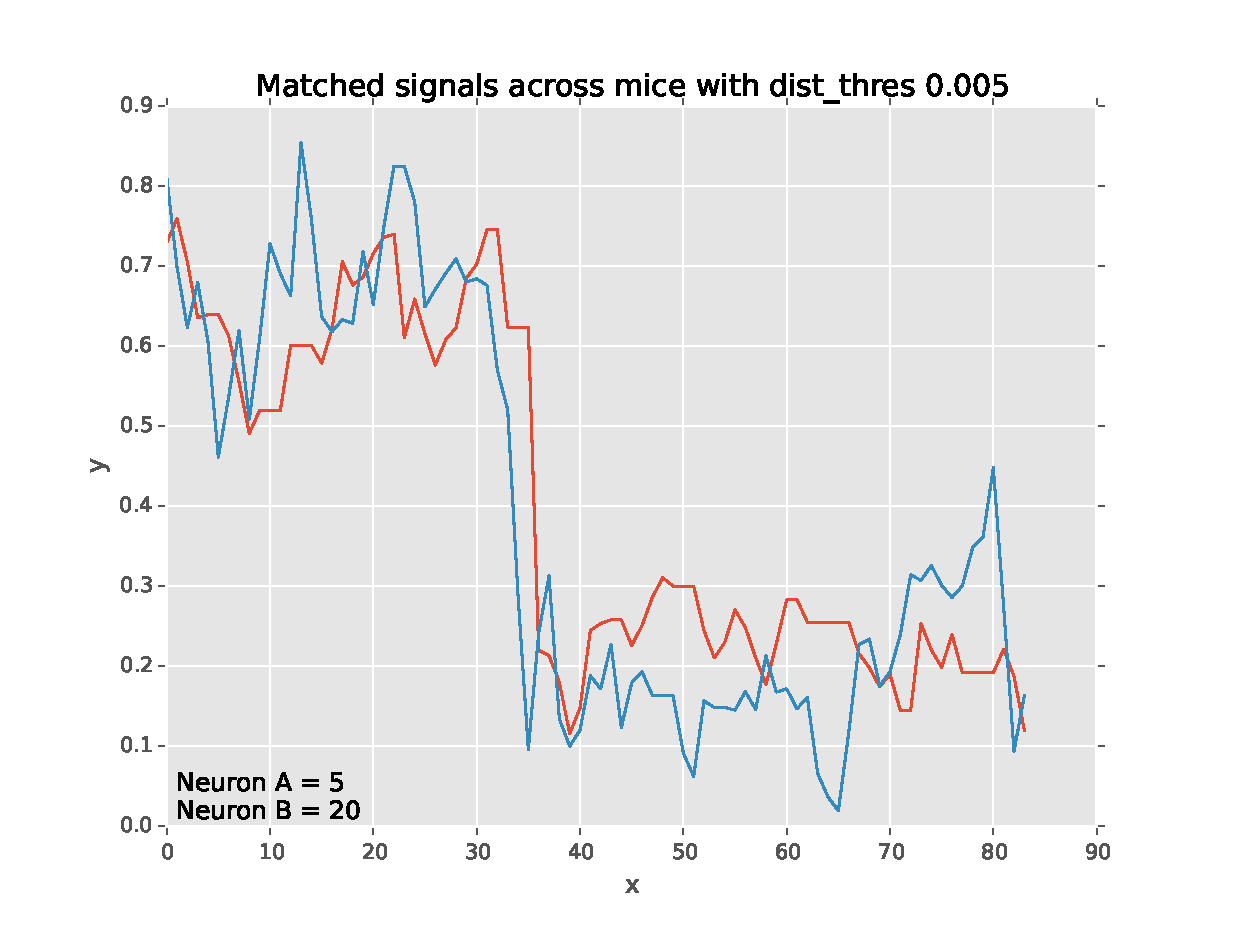
\includegraphics[width=\linewidth]{img/rlcsMain_getSegs_2016_04_12_08_09_50}
    \end{figure}

    \column{.5\textwidth} % Right column and width
    \begin{figure}
    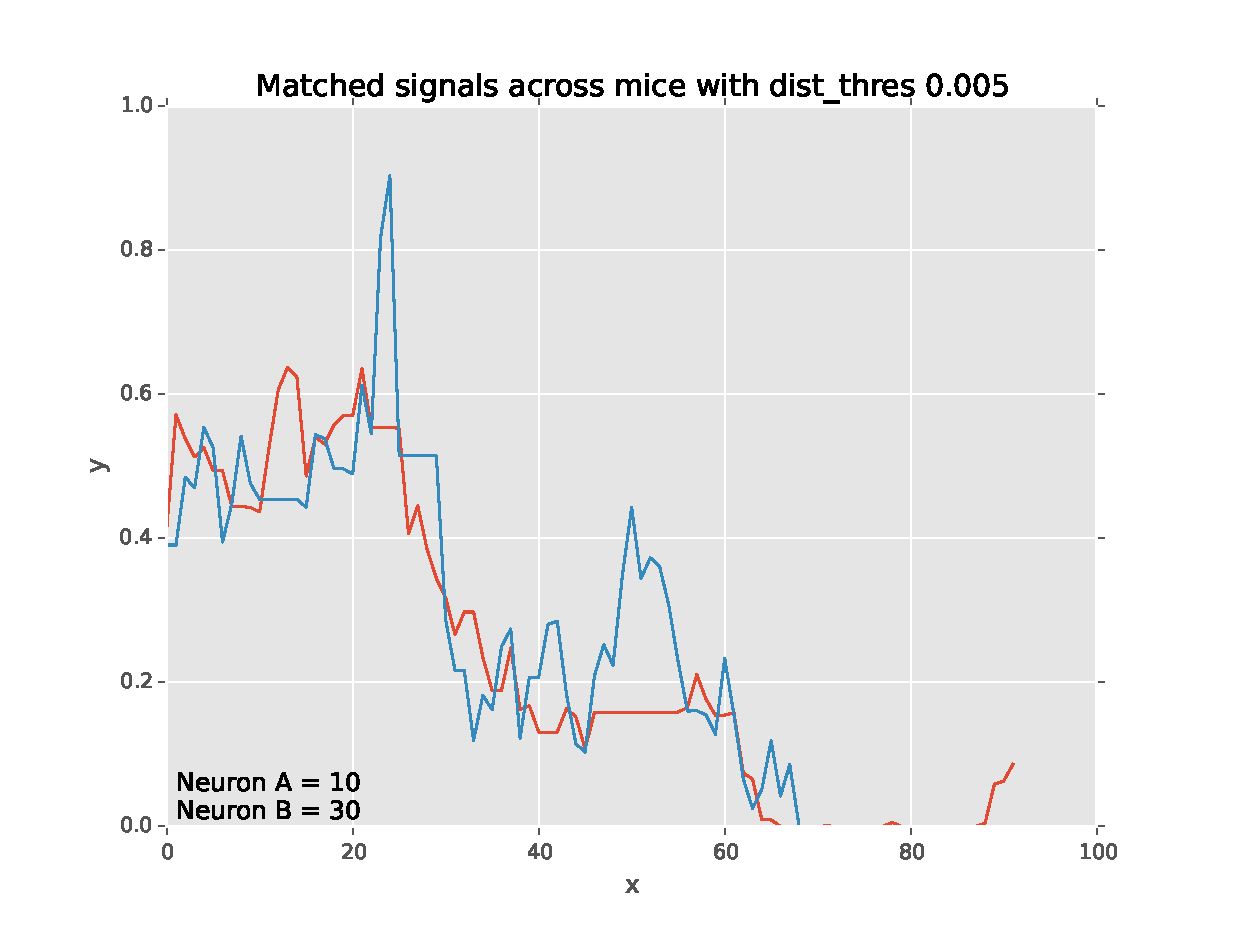
\includegraphics[width=\linewidth]{img/rlcsMain_getSegs_2016_04_12_08_12_31}
    \end{figure}
    \end{columns}
\end{frame}

\begin{frame}
\frametitle{Inferences}
\begin{itemize}
    \item Neuronal responses contain motifs/subsequences. The chemical process under every neuron's activation is same.
    \item Same neuron's response for different trial has a long subsequence. In every trial, receptive field of neuron stays approximately same.
    \item More or less any two neuron in the same mice contain motifs. On top of activation mechanism, neuronal interconnections could contribute to motifs.
    \item Motifs exists across neurons as well. But less frequent or motifs are shorter. As there are no neuronal connections, motifs across neurons are due to similar chemical activation process.
\end{itemize}
\end{frame}


%------------------------------------------------
\begin{frame}
\frametitle{References}
\footnotesize{
\begin{thebibliography}{99} % Beamer does not support BibTeX so references must be inserted manually as below

\bibitem[mark, 2014]{p1} Mark Mazurek, Marisa Kager and Stephen D. Van Hooser (2014)
\newblock Robust quantification of orientation selectivity and direction selectivity
\newblock \emph{Frontiers in Neural Circuits}.

\bibitem[Rikhye, 2015]{p1} Rajeev V. Rikhye and Mriganka Sur (2015)
\newblock Spatial Correlations in Natural Scenes Modulate Response Reliability in Mouse Visual Cortex
\newblock \emph{The Journal of Neuroscience}.

\bibitem[Smith, 2015]{p1} Shrey Dutta, Krishnaraj Sekhar PV and Hema A Murthy (2015)
\newblock Raga verification in carnatic music using longest common segment set
\newblock \emph{Journal Name} 12(3), 45 -- 678.

\bibitem[Dutta, 2013]{p1} Vignesh Ishwar, Shrey Dutta, Ashwin Bellur, Hema A Murthy (2013)
\newblock Motif Spotting in an Alapana in Carnatic Music.
\newblock \emph{ISMIR} 2013/11.

\bibitem[Dutta2, 2012]{p1} Shrey Dutta, Hema A Murthy (2014)
\newblock Discovering Typical Motifs of a Raga from One-Liners of Songs in Carnatic Music.
\newblock \emph{ISMIR}.
\end{thebibliography}
}
\end{frame}
%----------------------------------------------------------------------------------------

\end{document} 